\title{EN.601.448/648 Computational Genomics\\Final Project - Proposal}
\author{
        {Ayush Agarwal (aagarw33)}  \\
                Computer Science (Masters)\\
            \and
        {Lohita Sivaprakasam (lsivapr1)}  \\
                Computer Science (Masters)\\
                \and
        {Satish Palaniappan (spalani2)}  \\
                Computer Science (Masters)\\
                \and
        {Srivathsa Pasumarthi (psrivat1)}  \\
                Computer Science (Masters)\\
}
\date{\today}

\documentclass[12pt]{article}
\usepackage{graphicx}
\usepackage{wrapfig}
\usepackage{url}
\usepackage{wrapfig}
\usepackage{color}
\usepackage{marvosym}
\usepackage{enumerate}
\usepackage{subfigure}
\usepackage{tikz}
\usepackage[fleqn]{amsmath}
\usepackage{amssymb}
\usepackage{hyperref}
\usepackage[many]{tcolorbox}
\usepackage{lipsum}
\usepackage{float}
\usepackage{trimclip}
\usepackage{listings}
\usepackage{environ}
\usepackage{wasysym}
\usepackage{array}
\usepackage[margin=1in]{geometry}

\definecolor{blue}{rgb}{0,0,1}


\begin{document}
\maketitle

\section{Problem}

In this project, our primary aim is to perform taxonomic-classification of bacterial DNA
using various machine learning and deep learning approaches. The DNA sequences for these single-cell microorganisms serve as a unique identifier (like a barcode) for that species and characterizes each of them completely. Following \cite{src_work} as the base literature, we would like to perform the same classification using various other machine learning and deep learning approaches as described below and compare each method using defined metrics. Secondly, we would also like to use deep representation learning approaches to model meaningful representations of the DNA sequences and use these representations to perform hierarchical agglomerative clustering to validate if they correlate with their actual taxonomic hierarchy.

\section{Data}
We are using the same data as of \cite{src_work} which is from the Ribosomal Database Project (RDP \cite{rdp} -
{\color{blue}\href{https://rdp.cme.msu.edu/download/current_Bacteria_unaligned.fa.gz}{Download Link}}) and consists of around $\sim$550K samples of bacterial DNA along with the information about its taxa - phylum, class, order, family, genus. The source FASTA file was processed and samples whose sequence lengths were between 1270 and 1370 were picked; this choice was made only for keeping the sequence lengths almost constant while maximizing the total number of samples. The final data consists of $\sim$339K samples spanning over 3 phyla, 5 classes, 19 orders, 65 families and 393 genera. The processed CSV can be downloaded from {\color{blue}\href{https://www.dropbox.com/s/p7kb7aih0xurqxh/taxa.csv}{here}} and a snapshot of the data is shown in Figure 1.

\begin{figure}
\centering
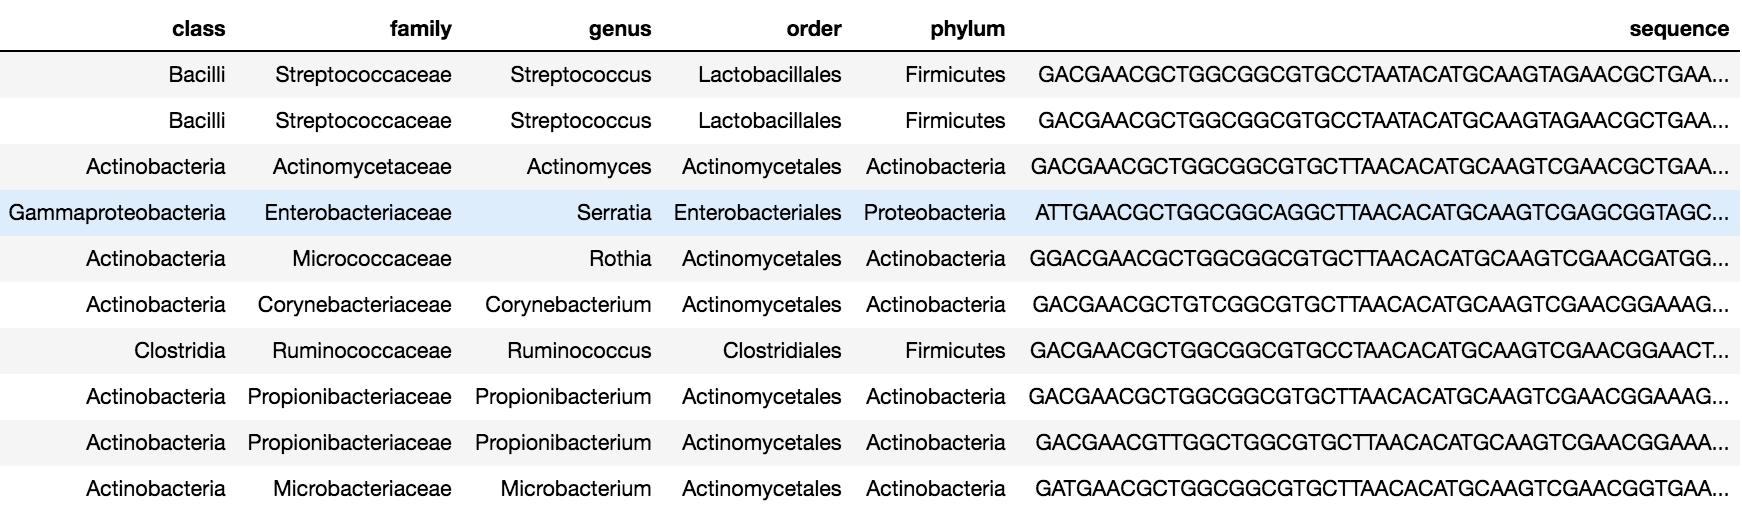
\includegraphics[scale=0.25]{data_snapshot.png}
\caption{A snapshot of the processed dataset}
\end{figure}

\section{Methods}
    \subsection{Methods for Taxonomic-Classification}
        \subsubsection{General Machine Learning methods (Features: k-mer counts)}
        We would like to use the k-mer counts of the DNA sequences as features and perform classification using general suite ML methods such as SVM, Random Forests, Naive-Bayes Classifier, KNN, etc. With these methods, we would like to grid search over different k values and find the best performing model, in order to determine the amount of context that is needed for taxonomy classification of the DNA sequences.
        \subsubsection{Convolutional Neural Networks (Features: QRCode-like image representation of DNA sequences)}
        Here we would like to explore an interesting way to represent a DNA sequence, which would be to visualize them as binary images, where the sequence is one-hot encoded over the ACGT base pairs. An example of this feature representation scheme is shown in Figure 2, for a sequence of length 30bp. We can then use this QRCode-like representation as an input to a convolutional neural network for performing taxonomy classification.

        \begin{figure}
        \centering
        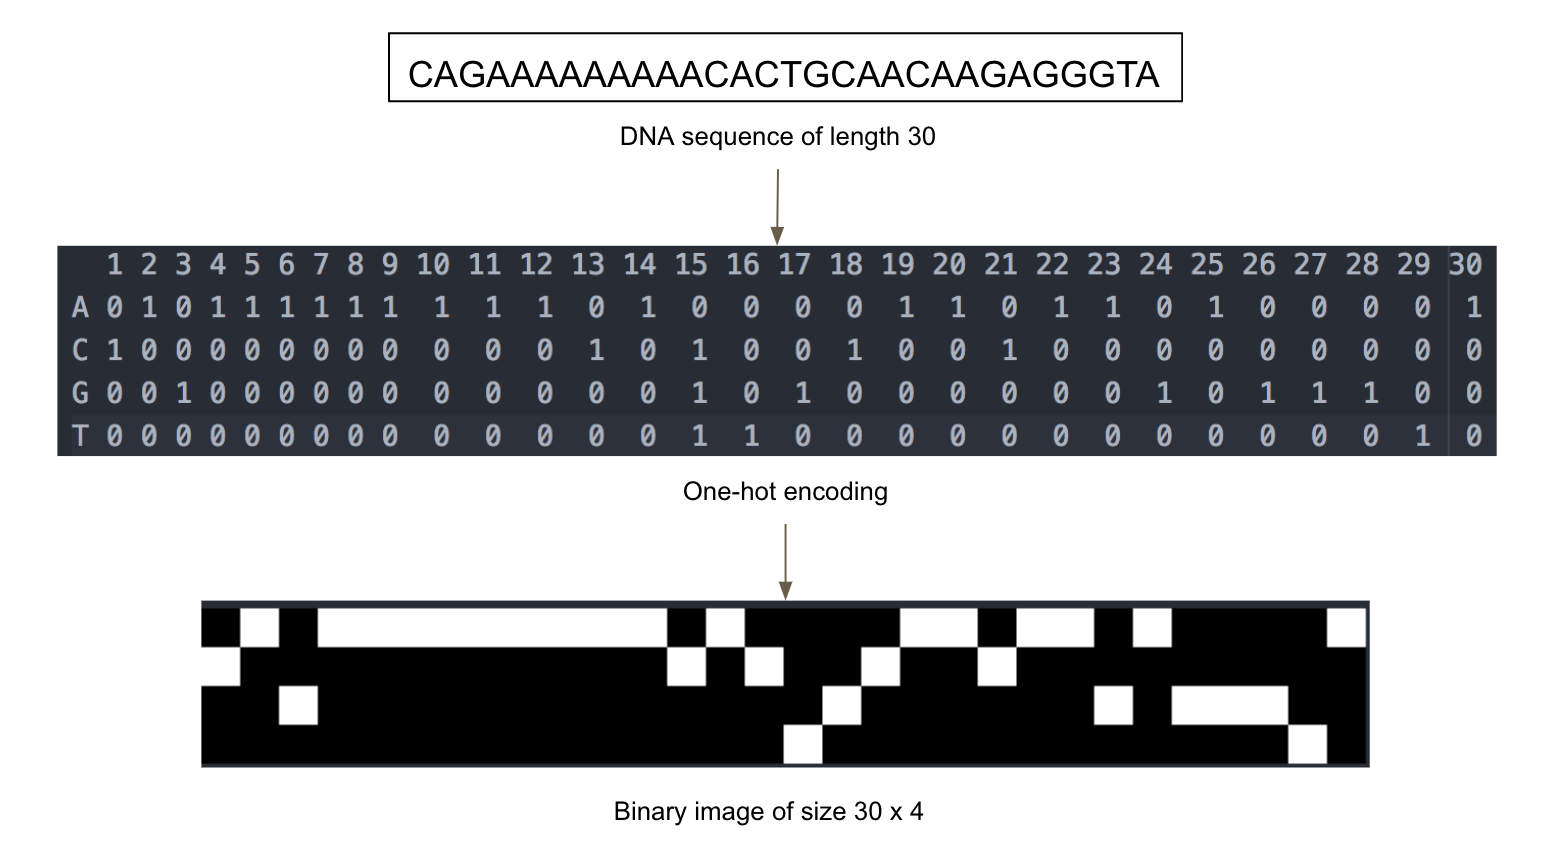
\includegraphics[scale=0.25]{qrcode.png}
        \caption{QR-code like DNA sequence representation}
        \end{figure}

        \subsubsection{Recurrent Neural Networks (Features: Raw DNA sequences)}
        Given the lack of explicit features and high dimensionality of the DNA sequences, recurrent neural networks provide an efficient way to encode the sequences for classification. Due to the ability of the Long Short Term Memory (LSTM) networks to process entire sequences and preserve the entire sequence's information irrespective of the gap length in huge sequences, an LSTM classifier can be used for the taxonomy classification of the input DNA sequences.

    \subsection{Representation Learning and Agglomerative Clustering}
    Deep representation learning has been used in recent years for various applications such as clustering, classification and data compression. Our goal here is to apply various representation learning techniques such as Variational Auto-Encoders (VAE) and LSTM Auto-Encoders to learn a representation of the DNA sequence and use that representation as features to perform hierarchical agglomerative clustering. The clustering is done to verify and validate that the learned representations actually correlate with their taxonomic hierarchy.
    \subsection{Ambitious Goals}
        These tasks will be done based on the availability of time and resources.
        \subsubsection{Ensemble Learning}
        We will attempt to learn multiple possibly uncorrelated learners to solve the same problem with sub-sampled data and combine these models to learn a meta-learner using stacking techniques such as an MLP, to get a much improved final prediction accuracy. This will help us leverage the advantages of multiple machine learning models.
        \subsubsection{Hybrid CNN-RNN approach}
        Here we borrow one of the key ideas from deep-learned image captioning architectures which use both CNNs and RNNs to learn representations of data and combine them into a richer lower dimension space to get a hybrid data representation that facilitates feature interaction among different types of data. Using this as key, we combine the QRCode-like representation of a DNA sequence run over a CNN and the raw DNA sequence run over an RNN using fully connected layers to finally perform taxonomy-classification, which we believe will give better results.

\section{Evaluation metrics}
We would like to use the following metrics used to evaluate any standard supervised classification or unsupervised clustering problem:
\begin{enumerate}
    \item \textbf{Classification Problem:} Overall accuracy, Per category accuracy, False Positive Rate, F1 score (Good metric for classification as it is the harmonic combination of precision and recall).
    \item \textbf{Clustering Problem:} Mutual Information Score, Homogeneity Score
\end{enumerate}

\section{Preliminary results}
We have done data cleaning, processing and Exploratory Data Analysis (EDA) where we have run simple queries to know the distribution under the different taxa. The Jupyter Notebook for pre-processing and EDA can be found {\color{blue}\href{https://nbviewer.jupyter.org/urls/dl.dropbox.com/s/862mx1q5jxsr5cl/EDA.ipynb}{here}}.

\section{Issues}
We foresee a few issues in this project which are enlisted below:
\begin{enumerate}
    \item Class imbalance at the family and genus level.
    \item Sequences are of a varied length which might be a challenge for CNN and RNN approaches. We are currently planning to truncate/pad to obtain sequences of fixed length, though there are ways to handle varying length sequences using RNNs which we will try.
    \item We are also skeptical about the deep representation learning approaches to actually model the distribution of each taxonomy-level groups.
\end{enumerate}

\begin{thebibliography}{9}
    \bibitem{src_work}
    Rizzo R., Fiannaca A., La Rosa M., Urso A.
    \textit{A Deep Learning Approach to DNA Sequence Classification}.
    Computational Intelligence Methods for Bioinformatics and Biostatistics. CIBB 2015.
    \bibitem{rdp}
    Cole, J. R., Q. Wang, J. A. Fish, B. Chai et al.
    \textit{Ribosomal Database Project: data and tools for high throughput rRNA analysis}.
    Nucl. Acids Res. 42(Database issue):D633-D642 2014
\end{thebibliography}

\end{document}
